\title{Proiect SGBD \\
- \\
Gestiunea unui magazin online}
\author{
    Dragancea Constantin \\
    Grupa 234
}
\date{}

\documentclass[12pt]{article}

\usepackage[utf8]{inputenc}
\usepackage[margin=1in]{geometry}
\usepackage[titletoc,title]{appendix}
\usepackage{amsmath,amsfonts,amssymb,mathtools}
\usepackage[ruled,vlined]{algorithm2e}
\usepackage{algorithmic}
\usepackage{xcolor}
\usepackage{listings}
\usepackage[dvipdfm]{graphicx}
    \graphicspath{ {./} }

\lstset{upquote=true}

\definecolor{codegreen}{rgb}{0,0.6,0}
\definecolor{codegray}{rgb}{0.5,0.5,0.5}
\definecolor{codepurple}{rgb}{0.58,0,0.82}
\definecolor{backcolour}{rgb}{0.95,0.95,0.92}

\lstdefinestyle{mystyle}{
    backgroundcolor=\color{backcolour},   
    commentstyle=\color{codegreen},
    keywordstyle=\color{magenta},
    numberstyle=\tiny\color{codegray},
    stringstyle=\color{codepurple},
    basicstyle=\ttfamily\footnotesize,
    breakatwhitespace=false,         
    breaklines=true,                 
    captionpos=b,                    
    keepspaces=true,                 
    numbers=left,                    
    numbersep=5pt,                  
    showspaces=false,                
    showstringspaces=false,
    showtabs=false,                  
    tabsize=2
}

\lstset{style=mystyle}

\begin{document}
\maketitle
\pagebreak

\tableofcontents
\pagebreak

\section{Introducere}
Pentru acest proiect, am ales să modelez o bază de date a unui magazin online. Aceasta cuprinde:
\begin{enumerate}
  \item Lista utilizatorilor de pe site
  \item Lista produselor, categoriilor și recenziilor produselor de pe site
  \item Posibilitatea de a plasa comenzi de mai multe produse și păstrarea informațiilor despre curierul acelei comenzi
  \item Lista depozitelor deținute de magazinul online
  \item Păstrarea informațiilor despre disponibilitatea unui produs într-un depozit
  \item Păstrarea unui tabel cu locații, ce poate fi folosit în mai multe contexte
\end{enumerate}

\pagebreak

\section{Diagrama E/R}

Diagrama Entitate Relație a modelului bazei de date este următoarea:

\begin{figure}[htp]
  \centering
  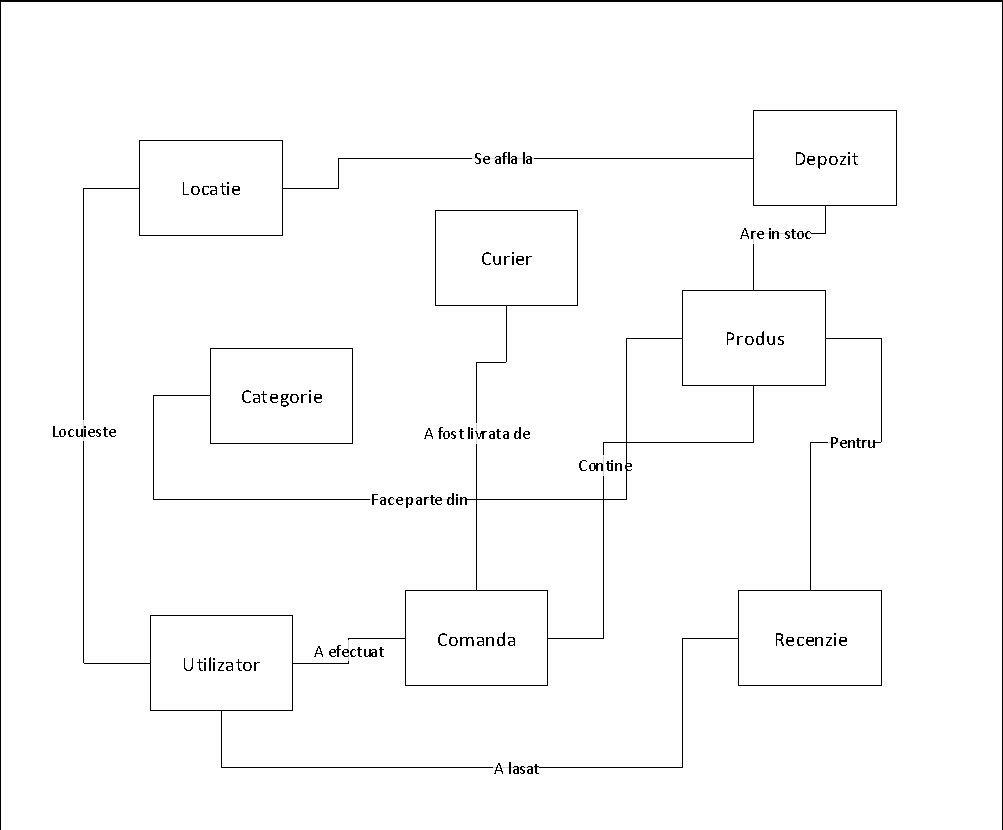
\includegraphics[width=1\linewidth]{EntitateRelatie.pdf}
  \caption{Diagrama Entitate/Relație}
\end{figure}

\pagebreak

\section{Diagrama Conceptuală}

Mai departe, am construit diagrama conceptuală a modelului, în care se evidențiază tabelele asociative necesare
rezolvării relațiilor \textit{many-to-many}, spre deosebire de diagrama E/R.

\begin{figure}[htp]
  \centering
  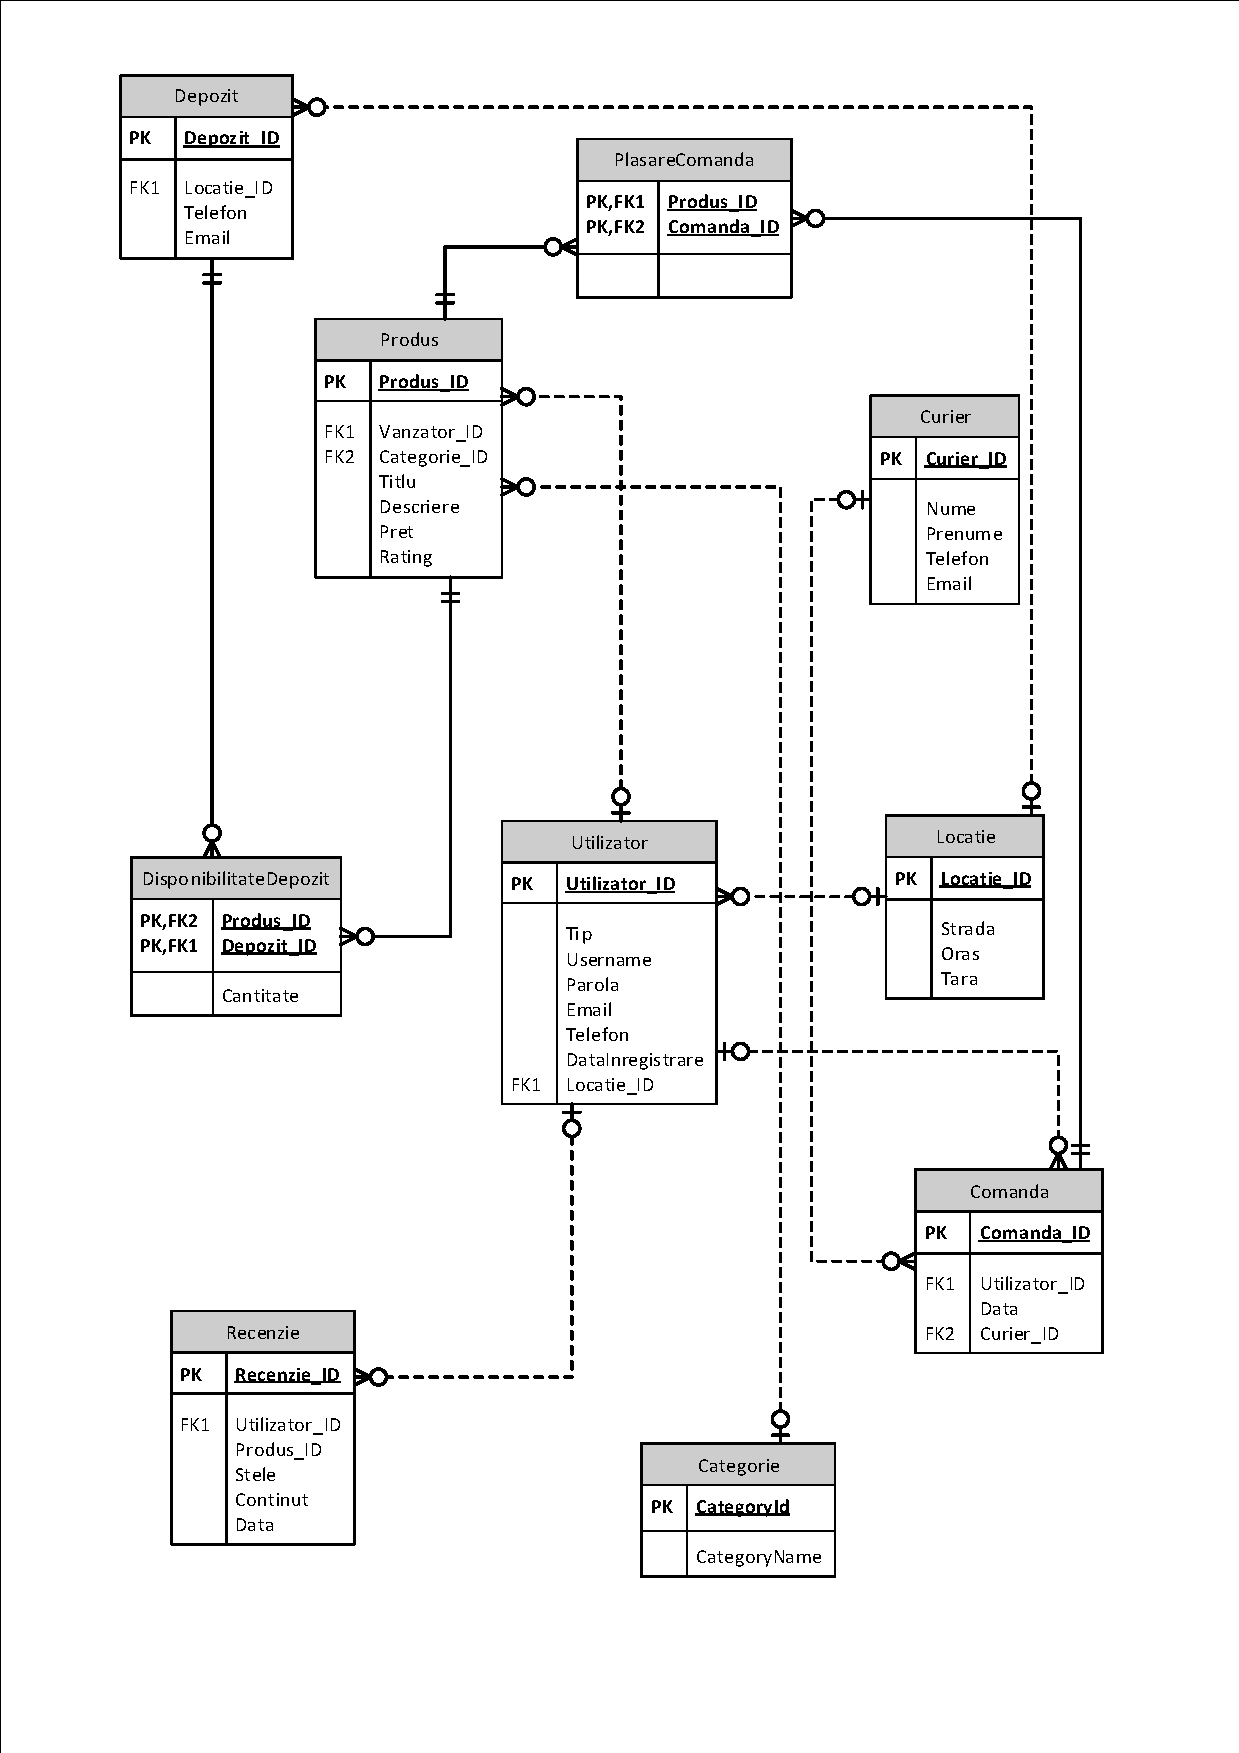
\includegraphics[width=0.72\linewidth]{DiagramaConceptuala.pdf}
  \caption{Diagrama Conceptuală}
\end{figure}

\pagebreak

\section{Crearea bazei de date}
Crearea bazei de date se rezumă la câteva insert-uri simple. Daca ținem cont de ordinea în care creăm tabelele,
putem sa definim si constrângerile de \textit{foreign key} în momentul creării tabelelor. Evident, trebuie să 
creăm tabelele care nu dețin chei străine în componența lor. De exemplu:

\vspace{0.5em}

\begin{lstlisting}[
  language=SQL,
  showspaces=false,
  basicstyle=\ttfamily,
  numbers=left,
  numberstyle=\tiny,
]
create table Locatie(
	locatie_id number primary key,
	adresa     varchar2(100),
	oras       varchar2(100),
	tara	   varchar2(100)
);
\end{lstlisting}

\vspace{0.5em}

Apoi adăugam tabele ce folosesc și chei externe, de exemplu:

\begin{lstlisting}[
  language=SQL,
  showspaces=false,
  basicstyle=\ttfamily,
  numbers=left,
  numberstyle=\tiny,
]
create table Utilizator(
	utilizator_id		number primary key,
	nume				varchar2(20) not null,
	prenume				varchar2(20),
	tip 				varchar2(20) not null,
	email				varchar2(60),
	telefon				varchar2(10),
	DataInregistrare	date,
	locatie_id			number not null,
	foreign key (locatie_id) references Locatie(locatie_id) on delete set null
);
\end{lstlisting}

\vspace{0.5em}

Iar la final adăugam și tabelele asociative, cum ar fi:

\vspace{0.5em}

\begin{lstlisting}[
  language=SQL,
  showspaces=false,
  basicstyle=\ttfamily,
  numbers=left,
  numberstyle=\tiny,
]
create table PlasareComanda(
	produs_id		number,
	comanda_id		number,
	cantitate		number,
	primary key (produs_id, comanda_id),
	foreign key (produs_id) references Produs(produs_id) on delete cascade,
	foreign key (comanda_id) references Comanda(comanda_id) on delete cascade
);
\end{lstlisting}

\pagebreak

\section{Popularea bazei de date}
Pentru a demonstra funcționalitatea bazei de date, aș fi putut scrie de mână câteva insert-uri, însă,
având ambiții de programator, am decis să găsesc o metodă mai "programatică" de a face acest lucru. Decât să 
iau date gata făcute de pe internet și să am bătăi de cap cu legile de protecție a datelor personale, voi
genera aceste intrări random. Uitându-mă peste diagrama conceptuală, am nevoie să generez următoarele tipuri
de informație: nume, prenume, adresă, orașe, țări, numere de telefon, email, dăți calendaristice, nume și descrieri
de produse, conținut de recenzii, nume de categorii. Pentru câmpurile formate din șiruri de caractere aș putea să creez efectiv
string-uri random, însă ar fi dificil de urmărit si analizat baza de date pentru o ființă umană. Cred că se 
poate mai bine de atât.

Voi apela la \textit{www.kaggle.com}, un website ce conține datasets din diverse domenii. Aici am găsit liste uriașe
cu nume și prenume uzuale în engleză. Astfel, pentru a alcătui numele și prenumele pentru o persoană, voi alege random 
din aceste 2 liste. Emailul personal îl pot construi după formatul nume.prenume@email.com . Numărul de telefon 
se generează ușor, atașând la prefixul 07 un număr de 8 cifre generat random.

Pentru adrese, pe același site am găsit un set, la fel de mare, cu adrese de stradă din SUA. Tot pe site, am
găsit și o colecție de orașe și țara căreia aparțin. Combinându-le, pot genera o intrare în tabelul \textit{Locatie}.

Pentru produse, am găsit o bază de date cu produse de pe un site de e-commerce indian, unde se afla și 
descrieri ale produselor. Pentru categorii, pot prelua un set de categorii de pe un magazin online existent, 
cum ar fi \textit{www.emag.ro}. Pentru recenzii, am găsit pe \textit{kaggle} o colecție de recenzii lăsate pe \textit{Amazon}.

Tot gândindu-mă cum sa generez niște date calendaristice random, am găsit un dataset cu răspunsuri lăsate pe
\textit{stackoverflow}, unde era inclus și timestamp-ul la care au fost lăsate, și am decis să le iau de acolo.


A fost o experiență bună să învăț să generez intrări random, pentru că acum pot cu ușurință sa modific cantitatea care
va fi generată. Dacă voi avea nevoie să fac niște \textit{stress tests}, adică să văd cât de bine se descurcă
baza mea de date din punct de vedere a eficieței timpului și spațiului, pot să o fac cu ușurință.

\pagebreak

\section{Cerința 6}
Pentru cerința 6, am implementat o procedură care va aplica o reducere de 5\% asupra produsului
cel mai puțin vândut în ultima lună. Logica sa este că magazinul vrea să își maximizeze fluxul de bani 
ce trece prin el, și va accepta un profit mai mic per unitate, în schimbul unei cantități mai mari vândute.
În caz de egalitate, adică dacă există mai multe produse care s-au vândut în aceeași cantitate minimă,
reducerea se va aplica tuturor acestor produse.
Pentru îndeplinirea acestei proceduri, am mai definit o funcție ce returneaza aceste produse vândute în cantitate 
minimă. În rezolvarea acestui exercițiu, am folosit un tablou indexat.

\vspace{0.5em}

\begin{lstlisting}[
  language=SQL,
  showspaces=false,
  basicstyle=\ttfamily,
  numbers=left,
  numberstyle=\tiny,
]
set serveroutput on;

create or replace procedure AplicaReducere
is
    type tablou      is table of number index by binary_integer;
    type tablou_imbr is table of number;
    Produse tablou_imbr;
    
    function AflaProduse
    return tablou_imbr
    is
        v       tablou;
        rasp    tablou_imbr:=tablou_imbr();
        mn      number;
    begin
        for prod in (
            select * from produs
        ) loop
            v(prod.produs_id) := 0;
        end loop;
        
        for vanzare in (
            select pc.* from PlasareComanda pc, comanda c
            where pc.comanda_id = c.comanda_id and
                months_between(sysdate, c.data) <= 1
        ) loop
            v(vanzare.produs_id) := v(vanzare.produs_id) + vanzare.cantitate;
        end loop;
        
        mn := v(v.first);
        for i in v.first .. v.last loop
            if v(i) < mn then
                mn := v(i);
                rasp.delete(rasp.first, rasp.last);
                rasp.extend;
                rasp(rasp.last) := i;
            elsif v(i) = mn then
                rasp.extend;
                rasp(rasp.last) := i;
            end if;
        end loop;
        
        return rasp;
    -- nu poate exista exceptia no data found, deoarece apelam functia 
    -- facand un group by inainte
    -- nu poate exista exceptia too many rows deoarece avem where rownum <= 1
    end AflaProduse;
    
begin
    Produse := AflaProduse;
    
    for i in Produse.first .. Produse.last loop
        update produs
        set pret = round(0.95 * pret, 2)
        where produs_id = Produse(i);
    end loop;
    commit;
end;
/

Execute AplicaReducere;
\end{lstlisting}

\pagebreak

\section{Cerința 7}
Magazinul nostru online vrea ca atunci când într-un depozit se află puține
unități ale unui produs, să organizeze o promoție de lichidare de stoc,
pentru a face loc pentru alte produse.
Astfel, are nevoie de o funcție, care la orice moment de timp, să afișeze
pentru fiecare produs id-ul depozitului ce conține cantitatea cea mai mică
de produs respectiv. Evident ne interesează doar depozitele care au măcar o
unitate de produs respectiv. Dacă un produs nu se află în nici o cantitate
în vreunul din depozite, nu i se poate organiza o promoție de lichidare de stoc, 
deci nu ne interesează. În această rezolvare folosesc un \textit{ciclu cursor}.

\vspace{0.5em}

\begin{lstlisting}[
  language=SQL,
  showspaces=false,
  basicstyle=\ttfamily,
  numbers=left,
  numberstyle=\tiny,
]
create or replace procedure LichidareStoc
is
    type tablou is table of number index by binary_integer;
    Depozite    tablou;
    prod_id      number;
    
    function DepozitCantitateMin(
        prod_id     number
    )
    return number
    is
        dep_id  number;
    begin
        select depozit_id
        into dep_id
        from (
            select * from DisponibilitateDepozit
            where produs_id = prod_id
            order by cantitate
        )
        where rownum <= 1;
        
        return dep_id;
    -- nu poate exista exceptia no data found, deoarece apelam functia 
    -- facand un group by inainte
    -- nu poate exista exceptia too many rows deoarece avem where
    -- rownum <= 1
    end DepozitCantitateMin;
    
begin
    for dp in (
        select produs_id from DisponibilitateDepozit
        group by produs_id) loop
        Depozite(dp.produs_id) := DepozitCantitateMin(dp.produs_id);
    end loop;
    
    for i in Depozite.first .. Depozite.last loop
        if Depozite.exists(i) then
            dbms_output.put_line('Produs id: '|| i||' Depozit id: '||Depozite(i));
        end if;
    end loop;
end;
/

Execute LichidareStoc;
\end{lstlisting}

\pagebreak

\section{Cerința 8}
Administratorii site-ului vor să știe pentru fiecare categorie de produse,
care e depozitul care deține cea mai mare cantitate de produse din acea
categorie.

Avem nevoie de tabelele Categorie, Produs, si DisponibilitateDepozit

\vspace{0.5em}

\begin{lstlisting}[
  language=SQL,
  showspaces=false,
  basicstyle=\ttfamily,
  numbers=left,
  numberstyle=\tiny,
]
-- Functia va returna numarul de Categorii care se regasesc in macar un depozit
create or replace function IdentificareDepozite
return number
is
    type tablou      is table of number index by binary_integer;
    type tablou_string is table of categorie.NumeCategorie%type index by binary_integer;
    Categorii        tablou;
    NumeCategorii    tablou_string;
    dep_id           number;
    ans              number := 0;
    
begin
    for categ in (
        select * from categorie
    ) loop
        NumeCategorii(categ.categorie_id) := categ.NumeCategorie;
        begin
            select depozit_id into dep_id
            from (
                select dp.depozit_id, sum(dp.cantitate) as numar_produse
                from produs p, DisponibilitateDepozit dp
                where p.categorie_id = categ.categorie_id and
                    dp.produs_id = p.produs_id
                group by dp.depozit_id
                order by numar_produse desc                    
            )
            where rownum <= 1;
            Categorii(categ.categorie_id) := dep_id;
        exception
            -- nu putem avea exceptia too many rows deoarece am un
            -- where rownum <= 1, deci putem avea maxim 1 rezultat
            when no_data_found then
                Categorii(categ.categorie_id) := null;
        end;
    end loop;
    
    for i in Categorii.first .. Categorii.last loop
        if Categorii(i) is null then
            dbms_output.put_line('Categoria '||NumeCategorii(i)||' nu se regaseste in niciun depozit');
        else
            dbms_output.put_line('Categoria: '|| NumeCategorii(i));
            dbms_output.put_line('Depozitul cu id-ul: '|| Categorii(i));
            ans := ans + 1;
        end if;
    end loop;
    return ans;
end;
/

begin
    dbms_output.put_line('Categorii care se regasesc in cel putin 1 depozit: '||IdentificareDepozite());
end;

-- Adaugam o categorie noua, astfel suntem siguri ca nu se regaseste
-- in niciun depozit
insert into categorie(categorie_id, NumeCategorie) values((select max(categorie_id) from categorie) + 1, 'CategorieNula');
begin
    dbms_output.put_line('Categorii care se regasesc in cel putin 1 depozit: '||IdentificareDepozite());
end;
rollback;
\end{lstlisting}

\pagebreak

\section{Cerința 9}
Magazinul are nevoie de o procedură care să afle valoarea comenzilor plasate de userii
dintr-un anumit oraș, în primele $k$ luni de la crearea contului

Avem nevoie de tabelele Locatie, Utilizator, Comanda, Produs si PlasareComanda

\vspace{0.5em}

\begin{lstlisting}[
  language=SQL,
  showspaces=false,
  basicstyle=\ttfamily,
  numbers=left,
  numberstyle=\tiny,
]
-- Functia va returna numarul de Categorii care se regasesc in macar un depozit
create or replace procedure VizualizareComenzi(
    nume_oras    locatie.oras%type,
    k            integer
)
is
    type tip_raspuns is record (utilizator_id   utilizator.utilizator_id%type,
                                nume            utilizator.nume%type,
                                prenume         utilizator.prenume%type,
                                valoare         number);
    type tablou is table of tip_raspuns;
    raspuns tablou;
    cnt     integer;
    
    function AflaPretProdus(
        prod_id     produs.produs_id%type
    ) return produs.pret%type
    is
        prod_pret   number;
    begin
        select pret into prod_pret
        from produs
        where produs_id = prod_id;
        
        return prod_pret;
    exception
        when no_data_found then
            raise_application_error(-20003, 'Nu exista produs cu id-ul dat in baza de date');
        -- nu putem avea exceptia too many rows doarece produs_id este cheie primara
    end AflaPretProdus;
    
    function AflaDataInregistrare(
        u_id    utilizator.utilizator_id%type
    ) return utilizator.DataInregistrare%type
    is
        dataReg     utilizator.DataInregistrare%type;
    begin
        select DataInregistrare into dataReg
        from utilizator
        where utilizator_id = u_id;
        
        return dataReg;
    exception
        when no_data_found then
            raise_application_error(-20000, 'Nu exista utilizator cu acest id');
        -- nu putem avea exceptia too many rows deoarece utilizator_id este cheie primara
    end AflaDataInregistrare;        
    
    function AflaValoareComenzi(
        u_id    utilizator.utilizator_id%type
    )
    return number
    is
        suma        number:=0;
        dataReg     date;
    begin   
        dataReg := AflaDataInregistrare(u_id);
        for my_comanda in (
            select pc.* from comanda c, PlasareComanda pc
            where utilizator_id = u_id and
                months_between(data, dataReg) <= k and
                c.comanda_id = pc.comanda_id
        ) loop
            suma := suma + my_comanda.cantitate * AflaPretProdus(my_comanda.produs_id);
        end loop;
        return suma;
    end AflaValoareComenzi;
begin
    select count(*) into cnt
    from locatie
    where oras = nume_oras;
    
    if cnt = 0 then
        raise_application_error(-20001, 'Nu exista oras cu numele dat in baza de date');
    end if;
    
    if k < 0 then
        raise_application_error(-20002, 'S-a dat un numar negativ de luni ca parametru');
    end if;
    
    select u.utilizator_id, u.nume, u.prenume, 0 as valoare
    bulk collect into raspuns
    from utilizator u, locatie l
    where l.oras = nume_oras and
        l.locatie_id = u.locatie_id;
    
    dbms_output.put_line('Valoarea comenzilor utilizatorilor din orasul '||nume_oras||
        ' in ultimele '||k||' luni');
    dbms_output.put_line('Id | Nume | Prenume | Valoarea comenzilor');
    for i in raspuns.first .. raspuns.last loop
        raspuns(i).valoare := AflaValoareComenzi(raspuns(i).utilizator_id);
        dbms_output.put_line(raspuns(i).utilizator_id||' '|| raspuns(i).nume||' '
            ||raspuns(i).prenume||' '||raspuns(i).valoare);
    end loop;
exception
    when no_data_found then
        raise_application_error(-20001, 'Nu exista oras cu numele dat in baza de date');
end;
/

-- trebuie pasat un oras care sa exista, sa consultam mai intai tabelul locatie
execute VizualizareComenzi('Tochigi', 100);

-- Dam un oras care nu exista
execute VizualizareComenzi('ABCD', 1);

-- Dam un numar negativ ca parametru pentru numarul de luni
execute VizualizareComenzi('Bucuresti', -1);
\end{lstlisting}

\pagebreak

\section{Cerința 10}
Magazinul își face totalurile activităților economice la sfârșitul fiecărui
trimestru. În momentul în care face aceste totaluri, vrem să ne asigurăm că
datele sunt consistente, astfel nu vrem ca o cumpărătură făcută să apară într-un
calcul, iar în altul nu (dacă de exemplu între completarile fișierelor/tabelelor excel
1 și 2 se mai face o comandă).
Soluția este ca în momentul în care se efectueaza aceste totaluri, să fie blocată
posbilitatea plasării unei comenzi. Totalurile se fac în cadrul orelor de lucru.

Astfel, în fiecare an, pe 31 martie, 30 iunie, 30 septembrie, 31 decembrie,
în intervalul de ore 9:00-17:00, este blocată posibilitatea plasării unei comenzi.

\vspace{0.5em}

\begin{lstlisting}[
  language=SQL,
  showspaces=false,
  basicstyle=\ttfamily,
  numbers=left,
  numberstyle=\tiny,
]
create or replace trigger SfarsitTrimestru
before insert or delete or update on PlasareComanda
begin
    if (to_char(sysdate, 'DD/MM') = '31/03' or
        to_char(sysdate, 'DD/MM') = '30/06' or
        to_char(sysdate, 'DD/MM') = '30/09' or
        to_char(sysdate, 'DD/MM') = '29/12') then
        
        raise_application_error(-20010, 'Plasarea/Modificarea/Stergerea comenzilor 
            este interzise in zilele in care se fac totalurile trimestrului!');
    end if;
end;
/

-- Pentru declansare incercam o inserare fie in una din cele 4 dati de mai sus,
-- fie adaugam in if sa verifice pentru ziua curenta
insert into PlasareComanda values(1, 3, 1);
\end{lstlisting}

\pagebreak

\section{Cerința 11}
Vrem să menținem în tabelul de categorii niște contoare a prețului minim,
respectiv maxim a unui produs din acea categorie.
Astfel, trebuie să avem grijă să modificam aceste campuri când se adaugă
un produs nou, sau modificâ unul existent, întrucât nu trebuie să fie
grija unui utilizator simplu a bazei de date.

Îl facem trigger de tip after ca să se faca automat check-urile constrângerii
de tip \textit{foreign key}

\vspace{0.5em}

\begin{lstlisting}[
  language=SQL,
  showspaces=false,
  basicstyle=\ttfamily,
  numbers=left,
  numberstyle=\tiny,
]
create or replace trigger categ_minmax_price
after insert or update on produs
for each row
declare
    min_pr      number;
    max_pr      number;
    categ       categorie%rowtype;
begin    
    min_pr := :new.pret;
    max_pr := :new.pret;
    
    select * into categ
    from categorie
    where categorie_id = :new.categorie_id;
    
    if nvl(categ.PretMinim, min_pr) < min_pr then
        min_pr := categ.PretMinim;
    end if;
    
    if nvl(categ.PretMaxim, max_pr) > max_pr then
        max_pr := categ.PretMaxim;
    end if;
    
    update categorie
    set PretMinim = min_pr,
        PretMaxim = max_pr
    where categorie_id = :new.categorie_id;
end;
/

-- Pentru declansare, inseram un produs nou
insert into Produs(produs_id, vanzator_id, categorie_id, titlu)
values ((select max(produs_id) from produs) + 1, 1, 1, 'Produs Test');
rollback;
\end{lstlisting}

\pagebreak

\section{Cerința 12}
Voi face un sistem de log-uri pentru baza de date. Pentru aceasta voi avea nevoie de un tabel în 
care să păstrez log-urile, un trigger ce să provoace scrierea în aceste log-uri, un director în care să 
scriu fișier-ul \textit{txt} de log-uri, privilegiile necesare de scriere, și trigger-ii ce să provoace
scrierea in acel fișier text.

\vspace{1em}

Mai întăi acord privilegiile necesare ca \textit{sysdba}.

\vspace{0.5em}

\begin{lstlisting}[
  language=SQL,
  showspaces=false,
  basicstyle=\ttfamily,
  numbers=left,
  numberstyle=\tiny,
]
grant execute on utl_file to constantin;
-- permite folosirea pachetului utl_file, ce are definite functii de IO cu fisier

grant execute on dbms_sql to constantin;
-- permite folosirea pachetului dbms_sql, pentru a putea deschide cursori in modul necesar noua

create directory logs as 'E:\OracleLogs';
-- creaza folder-ul unde vor fi scrise log-urile;

grant read, write on directory logs to constantin;
-- da privilegiile necesare pentru a putea face operatii de IO in acel directory
\end{lstlisting}

\vspace{0.5em}

Acum trebuie să implementez tabelele în care voi păstra intrările de log-uri și trigger-ul ce va
efectua scrierea în acest tabel:

\vspace{0.5em}

\begin{lstlisting}[
  language=SQL,
  showspaces=false,
  basicstyle=\ttfamily,
  numbers=left,
  numberstyle=\tiny,
]
create table audit_user(
    nume_bd             varchar2(50),
    user_logat          varchar2(30),
    eveniment           varchar2(100),
    tip_obiect_referit  varchar2(100),
    nume_obiect_referit varchar2(100),
    data                timestamp(3),
    nr_tabele           integer,
    nr_triggere         integer
);
/
create or replace trigger audit_schema
after create or drop or alter on schema
begin
    insert into audit_user values(
        sys.database_name,
        sys.login_user,
        sys.sysevent,
        sys.dictionary_obj_type,
        sys.dictionary_obj_name,
        systimestamp(3),
        (select count(*) from user_tables),
        (select count(*) from user_triggers)
    );
end;
/
\end{lstlisting}

\vspace{0.5em}

Combinând acest trigger cu unul care să scrie într-un fișier aceste log-uri
atunci când user-ul iese, sau baza de date se închide sau întâmpină o
eroare, o sa avem aceste log-uri fără nevoia de a mai intra înapoi in baza
de date.

\vspace{0.5em}

\begin{lstlisting}[
  language=SQL,
  showspaces=false,
  basicstyle=\ttfamily,
  numbers=left,
  numberstyle=\tiny,
]
-- vom defini o functie ce o vom utiliza in urmatoarele triggere
-- dupa executarea acestei functii, in directorul si fisierul cu numele specificat, se va afla
-- continutul tabelului audit_schema
create or replace procedure writelogs
is
    fisier  utl_file.file_type;
    p_sql_query varchar2(300):='select 
        nume_bd, user_logat, eveniment, tip_obiect_referit,
        nume_obiect_referit, data, nr_tabele, nr_triggere
    from audit_user';
    l_cursor_handle integer;
    l_dummy         number;
    l_rec_tab       dbms_sql.desc_tab;
    l_col_cnt       integer;
    l_current_line  varchar(2047);
    l_current_col   number(16);
    l_record_count  number(16):=0;
    l_column_value  varchar2(300);
    l_print_text    varchar2(300);
begin
    -- deschide fisierul pentru write
    fisier := utl_file.fopen('LOGS', 'logs.txt', 'w', 2047);
    
    -- deschide un cursor cu selectul din audit_user
    l_cursor_handle := dbms_sql.open_cursor;
    dbms_sql.parse(l_cursor_handle, p_sql_query, dbms_sql.native);
    l_dummy := dbms_sql.execute(l_cursor_handle);
    
    -- afla numele coloanelor
    dbms_sql.describe_columns(l_cursor_handle, l_col_cnt, l_rec_tab);
    
    -- append to file column headers
    l_current_col := l_rec_tab.first;
    if (l_current_col is not null) then
        loop
            dbms_sql.define_column(l_cursor_handle, l_current_col, l_column_value, 300);
            l_print_text := l_rec_tab(l_current_col).col_name || ' ';
            utl_file.put(fisier, l_print_text);
            l_current_col := l_rec_tab.next(l_current_col);
            exit when (l_current_col is null);
        end loop;
    end if;
    utl_file.put_line(fisier, ' ');
    
    -- append data for each row
    loop
        exit when dbms_sql.fetch_rows(l_cursor_handle) = 0;
        
        l_current_line := '';
        for l_current_col in 1..l_col_cnt loop
            dbms_sql.column_value(l_cursor_handle, l_current_col, l_column_value);
            l_print_text := l_column_value;
            
            l_current_line := l_current_line || l_column_value || ' ';
        end loop;
        
        l_record_count := l_record_count + 1;
        utl_file.put_line(fisier, l_current_line);
    end loop;
    
    utl_file.fclose(fisier);
    dbms_sql.close_cursor(l_cursor_handle);
    
exception
    when others then
        -- eliberam resursele de sistem
        if dbms_sql.is_open(l_cursor_handle) then
            dbms_sql.close_cursor(l_cursor_handle);
        end if;
        
        if utl_file.is_open(fisier) then
            utl_file.fclose(fisier);
        end if;
        
        dbms_output.put_line(dbms_utility.format_error_stack);
end;
/

create or replace trigger logoff_write_logs
before logoff on schema
begin
    writelogs;
end;
/

create or replace trigger log_erori
after servererror on schema
begin
    writelogs;
end;
/

create or replace trigger shutdown_write_logs
before shutdown on schema
begin
    writelogs;
end;
/
\end{lstlisting}

\pagebreak

\section{Cerința 13}

\vspace{0.5em}

\begin{lstlisting}[
  language=SQL,
  showspaces=false,
  basicstyle=\ttfamily,
  numbers=left,
  numberstyle=\tiny,
]
create or replace package proiect
is
    type tablou         is table of number index by binary_integer;
    type tablou_imbr    is table of number;
    type tip_rasp_com   is record(
        utilizator_id   utilizator.utilizator_id%type,
        nume            utilizator.nume%type,
        prenume         utilizator.prenume%type,
        valoare         number);
    type tablou_raspuns is table of tip_rasp_com;
    
    procedure AplicaReducere;
    
    function AflaProduse return tablou_imbr;
    
    procedure LichidareStoc;
    
    function DepozitCantitateMin(
        prod_id     number
    ) return number;
    
    procedure VizualizareComenzi(
        nume_oras   locatie.oras%type,
        k           integer);
    
    function AflaPretProdus(
        prod_id     produs.produs_id%type
    ) return produs.pret%type;
    
    function AflaValoareComenzi(
        u_id        utilizator.utilizator_id%type,
        k           integer
    ) return number;
end proiect;
/

create or replace package body proiect
is
    function AflaProduse
    return tablou_imbr
    is
        v       tablou;
        rasp    tablou_imbr:=tablou_imbr();
        mn      number;
    begin
        for prod in (
            select * from produs
        ) loop
            v(prod.produs_id) := 0;
        end loop;
        
        for vanzare in (
            select pc.* from PlasareComanda pc, Comanda c
            where pc.comanda_id = c.comanda_id and
                months_between(sysdate, c.data) <= 1
        ) loop
            v(vanzare.produs_id) := v(vanzare.produs_id) + vanzare.cantitate;
        end loop;
        
        mn := v(v.first);
        for i in v.first .. v.last loop
            if v(i) < mn then
                rasp.delete(rasp.first, rasp.last);
                rasp.extend;
                rasp(rasp.last) := i;
            elsif v(i) = mn then
                rasp.extend;
                rasp(rasp.last) := i;
            end if;
        end loop;
        
        return rasp;
    end Aflaproduse;
    
    procedure AplicaReducere
    is
        Produse     tablou_imbr;
    begin
        Produse := AflaProduse;
        
        for i in Produse.first .. Produse.last loop
            update produs
            set pret = round(0.95 * pret, 2)
            where produs_id = Produse(i);
        end loop;
        commit;
    end AplicaReducere;
    
    function DepozitCantitateMin(
        prod_id     number
    ) return number
    is
        dep_id  number;
    begin
        select depozit_id into dep_id
        from (
            select * from DisponibilitateDepozit
            where produs_id = prod_id
            order by cantitate
        )
        where rownum <= 1;
        
        return dep_id;
    exception
        when no_data_found then
            raise_application_error(-20020, 'Produsul dat nu se gaseste in
                niciun depozit');
    end DepozitcantitateMin;
    
    procedure LichidareStoc
    is
        Depozite    tablou;
        prod_id     number;
    begin
        for dp in (
            select produs_id from DisponibilitateDepozit
            group by produs_id) loop
            
            Depozite(dp.produs_id) := DepozitCantitateMin(dp.produs_id);
        end loop;
        
        for i in Depozite.first .. Depozite.last loop
            if Depozite.exists(i) then
                dbms_output.put_line('Produs id: '||i||' Depozit id: '||Depozite(i));
            end if;
        end loop;
    end LichidareStoc;
    
    function AflaPretProdus(
        prod_id     produs.produs_id%type
    ) return produs.pret%type
    is
        prod_pret   number;
    begin
        select pret into prod_pret
        from produs
        where produs_id = prod_id;
        
        return prod_pret;
    exception
        when no_data_found then
            raise_application_error(-20021, 'Nu exista produs cu id-ul dat');
    end AflaPretProdus;
    
    function AflaDataInregistrare(
        u_id    utilizator.utilizator_id%type
    ) return utilizator.DataInregistrare%type
    is
        dataReg     utilizator.DataInregistrare%type;
    begin
        select DataInregistrare into dataReg
        from utilizator
        where utilizator_id = u_id;
        
        return dataReg;
    exception
        when no_data_found then
            raise_application_error(-20022, 'Nu exista utilizator cu acest id');
    end AflaDataInregistrare;
    
    function AflaValoareComenzi(
        u_id    utilizator.utilizator_id%type,
        k       integer
    ) return number
    is
        suma    number:=0;
        dataReg date;
    begin
        dataReg := AflaDataInregistrare(u_id);
        for my_comanda in (
            select pc.* from comanda c, PlasareComanda pc
            where utilizator_id = u_id and
                months_between(data, dataReg) <= k and
                c.comanda_id = pc.comanda_id
        ) loop
            suma := suma + my_comanda.cantitate * AflaPretProdus(my_comanda.produs_id);
        end loop;
        
        return suma;
    end AflaValoareComenzi;
    
    procedure VizualizareComenzi(
        nume_oras       locatie.oras%type,
        k               integer)
    is
        raspuns     tablou_raspuns;
        cnt         integer;
    begin
        select count(*) into cnt
        from locatie
        where oras = nume_oras;
        
        if cnt = 0 then
            raise_application_error(-20023, 'Nu exista oras cu numele dat in baza de date');
        end if;
        
        if k < 0 then
            raise_application_error(-20024, 'S-a dat un numar negativ de luni ca parametru');
        end if;
        
        select u.utilizator_id, u.nume, u.prenume, 0 as valoare
        bulk collect into raspuns
        from utilizator u, locatie l
        where l.oras = nume_oras and
            l.locatie_id = u.locatie_id;
        
        dbms_output.put_line('Valoarea comenzilor utilizatorilor din orasul '||nume_oras||
            ' in ultimele '||k||' luni');
        dbms_output.put_line('Id | Nume | Prenume | Valoarea comenzilor');
        for i in raspuns.first .. raspuns.last loop
            raspuns(i).valoare := AflaValoareComenzi(raspuns(i).utilizator_id, k);
            dbms_output.put_line(raspuns(i).utilizator_id||' '|| raspuns(i).nume||' '
                ||raspuns(i).prenume||' '||raspuns(i).valoare);
        end loop;
    exception
    when no_data_found then
        raise_application_error(-20001, 'Nu exista oras cu numele dat in baza de date');
    end VizualizareComenzi;
end proiect;
/
\end{lstlisting}

\pagebreak

\section{Cerința 14}
Pentru cerința 14 am scris un pachet capabil să scrie conținutul unui tabel specificat într-un fișier specificat.

\begin{lstlisting}[
language=SQL,
showspaces=false,
basicstyle=\ttfamily,
numbers=left,
numberstyle=\tiny,
]
-- Cerinta 14

-- Un pachet ce contine functiile necesare pentru a scrie continutul unui tabel intr-un fisier

create or replace package wfile
is
    procedure write_to_file(
        nume_tabel      user_tables.table_name%type,
        nume_fisier     varchar2
    );
    
    procedure check_table_exists(
        nume_tabel  user_tables.table_name%type
    );
end wfile;
/

create or replace package body wfile
is
    procedure check_table_exists(
        nume_tabel   user_tables.table_name%type
    )
    is
        cnt integer;
    begin
        select count(*) into cnt
        from user_tables
        where lower(table_name) = lower(nume_tabel);
        
        if (cnt = 0) then
            raise_application_error(-20050, 'Nu exista acest tabel in user space');
        end if;
        return;
    end check_table_exists;
    
    procedure write_to_file(
        nume_tabel      user_tables.table_name%type,
        nume_fisier     varchar2)
    is
        fisier          utl_file.file_type;
        p_sql_query     varchar2(300):='select * from ';
        l_cursor_handle integer;
        l_dummy         number;
        l_rec_tab       dbms_sql.desc_tab;
        l_col_cnt       integer;
        l_current_line  varchar(2047);
        l_current_col   number(16);
        l_record_count  number(16):=0;
        l_column_value  varchar2(300);
        l_print_text    varchar2(300);
    begin
        check_table_exists(nume_tabel);
    
        p_sql_query := p_sql_query || nume_tabel;
        -- deschide fisierul pentru write
        -- LOGS reprezinta un directory creat din sql, ce are incorporata si adresa pe disk unde se va scrie fisierul
        -- pentru a scrie in alta locatie, trebuie sa declaram acel directory, si sa acordam drepturi de read-write
        -- utilizatorului pentru acel fisier
        fisier := utl_file.fopen('LOGS', nume_fisier, 'w', 2047);
        
        -- deschide un cursor cu selectul din audit_user
        l_cursor_handle := dbms_sql.open_cursor;
        dbms_sql.parse(l_cursor_handle, p_sql_query, dbms_sql.native);
        l_dummy := dbms_sql.execute(l_cursor_handle);
        
        -- afla numele coloanelor
        dbms_sql.describe_columns(l_cursor_handle, l_col_cnt, l_rec_tab);
        
        -- append to file column headers
        l_current_col := l_rec_tab.first;
        if (l_current_col is not null) then
            loop
                dbms_sql.define_column(l_cursor_handle, l_current_col, l_column_value, 300);
                l_print_text := l_rec_tab(l_current_col).col_name || ' ';
                utl_file.put(fisier, l_print_text);
                l_current_col := l_rec_tab.next(l_current_col);
                exit when (l_current_col is null);
            end loop;
        end if;
        utl_file.put_line(fisier, ' ');
        
        -- append data for each row
        loop
            exit when dbms_sql.fetch_rows(l_cursor_handle) = 0;
            
            l_current_line := '';
            for l_current_col in 1..l_col_cnt loop
                dbms_sql.column_value(l_cursor_handle, l_current_col, l_column_value);
                l_print_text := l_column_value;
                
                l_current_line := l_current_line || l_column_value || ' ';
            end loop;
            
            l_record_count := l_record_count + 1;
            utl_file.put_line(fisier, l_current_line);
        end loop;
        
        utl_file.fclose(fisier);
        dbms_sql.close_cursor(l_cursor_handle);
        
    exception
        when others then
            -- eliberam resursele de sistem
            if dbms_sql.is_open(l_cursor_handle) then
                dbms_sql.close_cursor(l_cursor_handle);
            end if;
            
            if utl_file.is_open(fisier) then
                utl_file.fclose(fisier);
            end if;
            
            dbms_output.put_line(dbms_utility.format_error_stack);
    end write_to_file;
    
end wfile;
/


Execute wfile.write_to_file('audit_user', 'test.txt');
/
\end{lstlisting}

\section{Concluzii}
În acest proiect am reușit sa modelez activitatea unui magazin online și să valorific cunoștințele mele în 
\textit{SQL} și \textit{PL/SQL}. Am implementat proceduri și funcții, am folosit tipuri de date și obiecte 
complexe precum record, tabel index, tabel imbricat și cursor.

Alături de acest pdf, se vor mai găsi și fișierele aferente bazei de date:

\begin{itemize}
  \item \textit{createDatabase.sql} - crearea tabelelor, constrângerilor și trigger-ilor necesare modelului
  \item \textit{populateDatabase.sql} - script-ul de populare a bazei de date cu niște date exemplu, pentru
        a putea testa subprogramele create
  \item \textit{Cerintai.sql} - fișierul ce conține implementarea cerinței $i$
  \item \textit{PopulateDatabase.py} - un script \textit{Python} folosit pentru adăugarea inserărilor random
        în baza de date.
  \item \textit{PopulateDatabase.sql} - script-ul \textit{SQL} produs de cel de mai sus ce conține insert-urile propriu-zise
\end{itemize}

\pagebreak


\section{Screenshots}

\begin{figure}[htp]
\centering
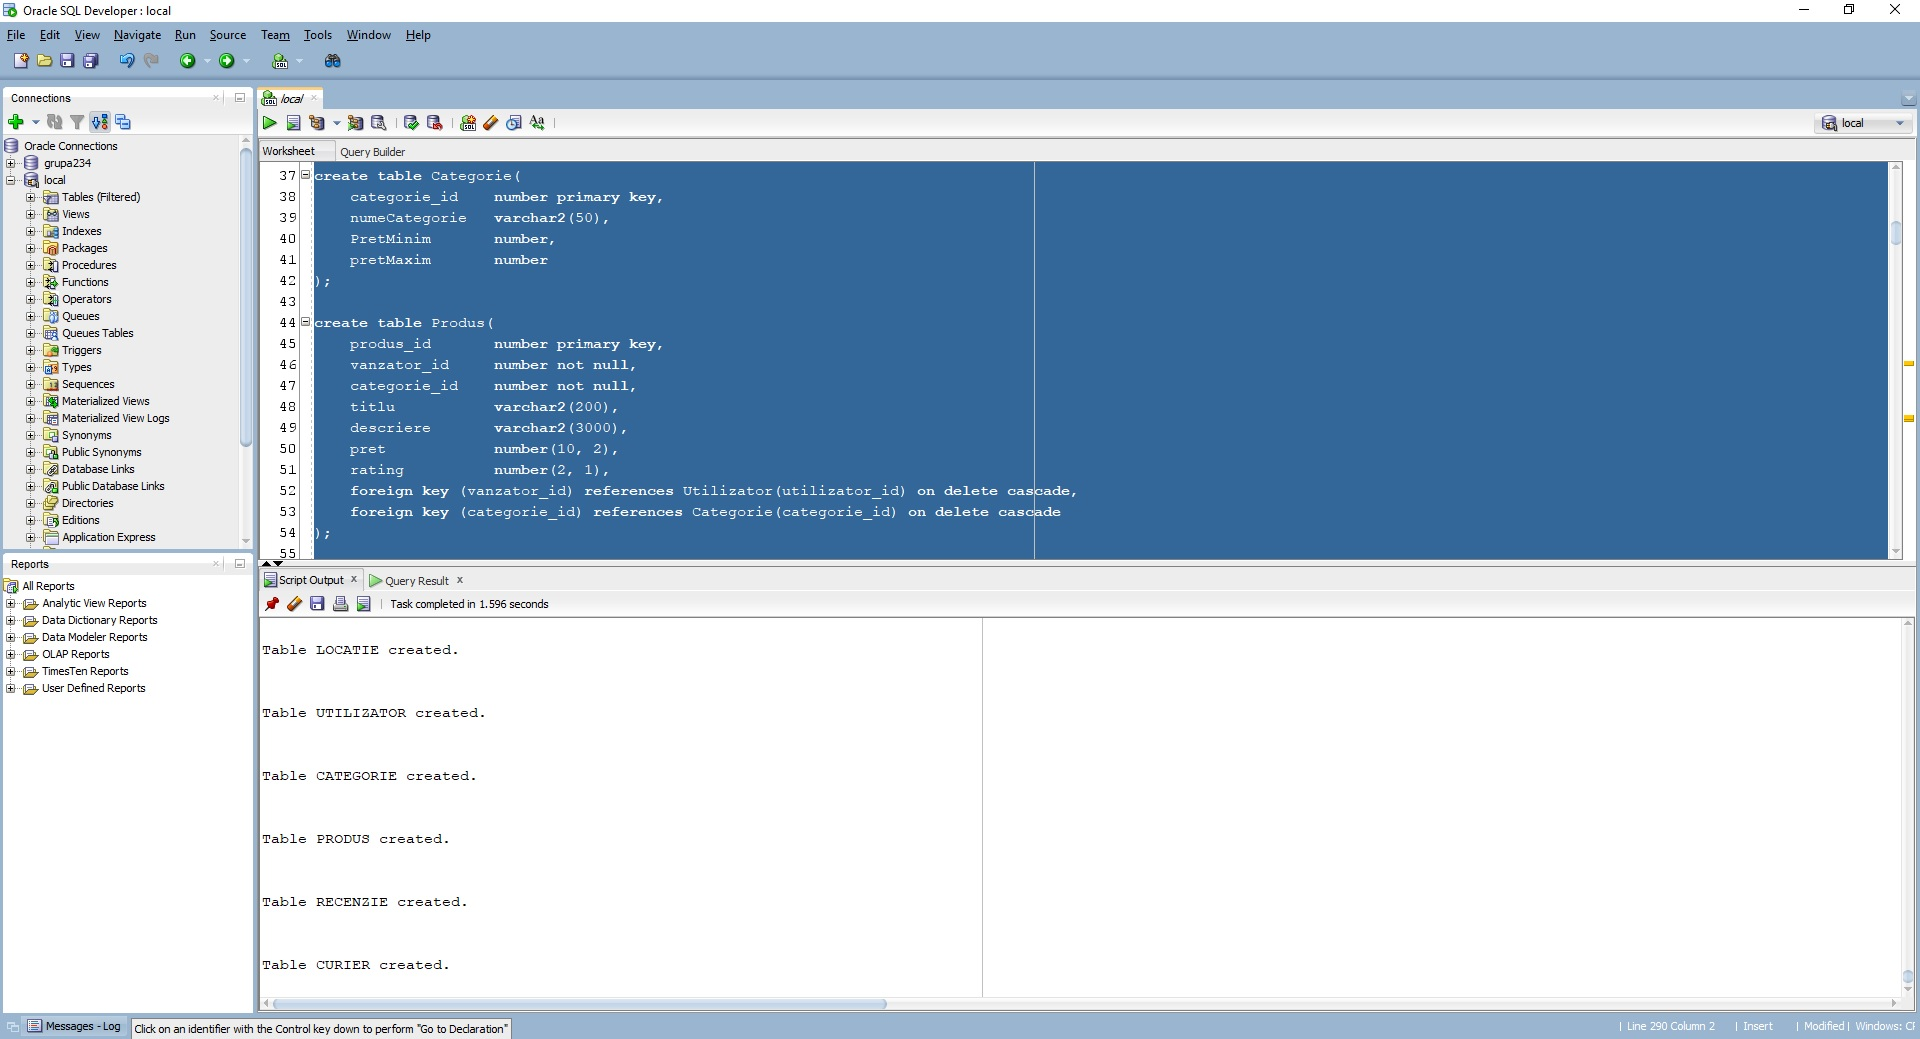
\includegraphics[width=1\linewidth]{Creare.jpg}
\caption{Crearea bazei de date}
\end{figure}

\begin{figure}[htp]
\centering
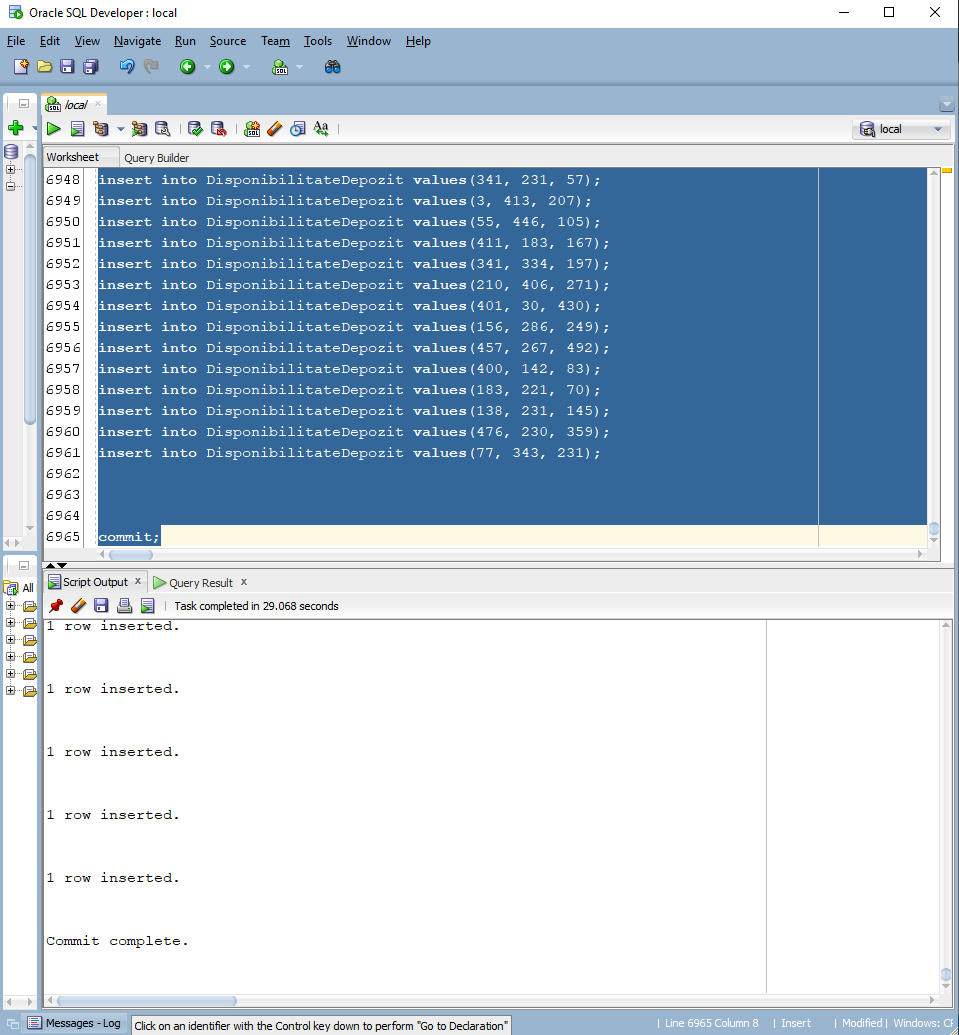
\includegraphics[width=1\linewidth]{Populare.png}
\caption{Popularea bazei de date}
\end{figure}

\begin{figure}[htp]
\centering
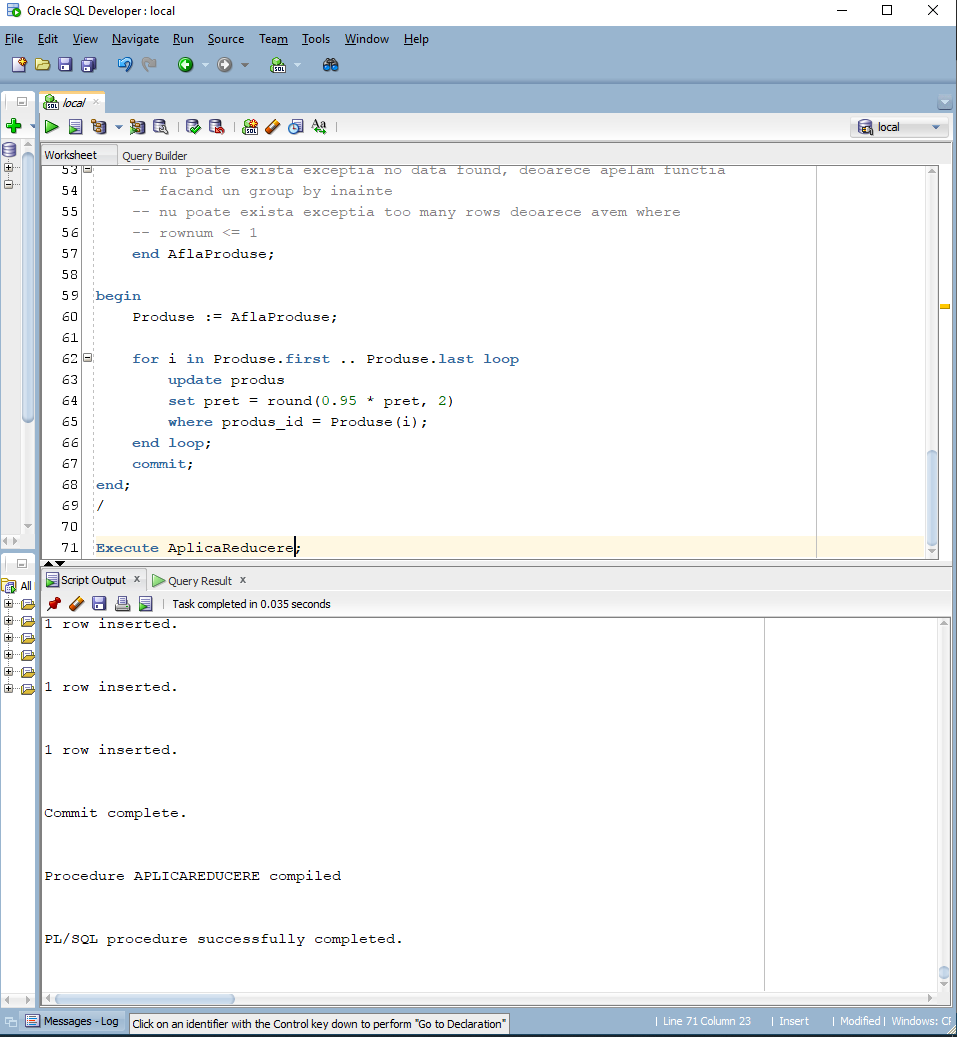
\includegraphics[width=1\linewidth]{Cerinta6.png}
\caption{Execuția cerinței 6}
\end{figure}

\begin{figure}[htp]
\centering
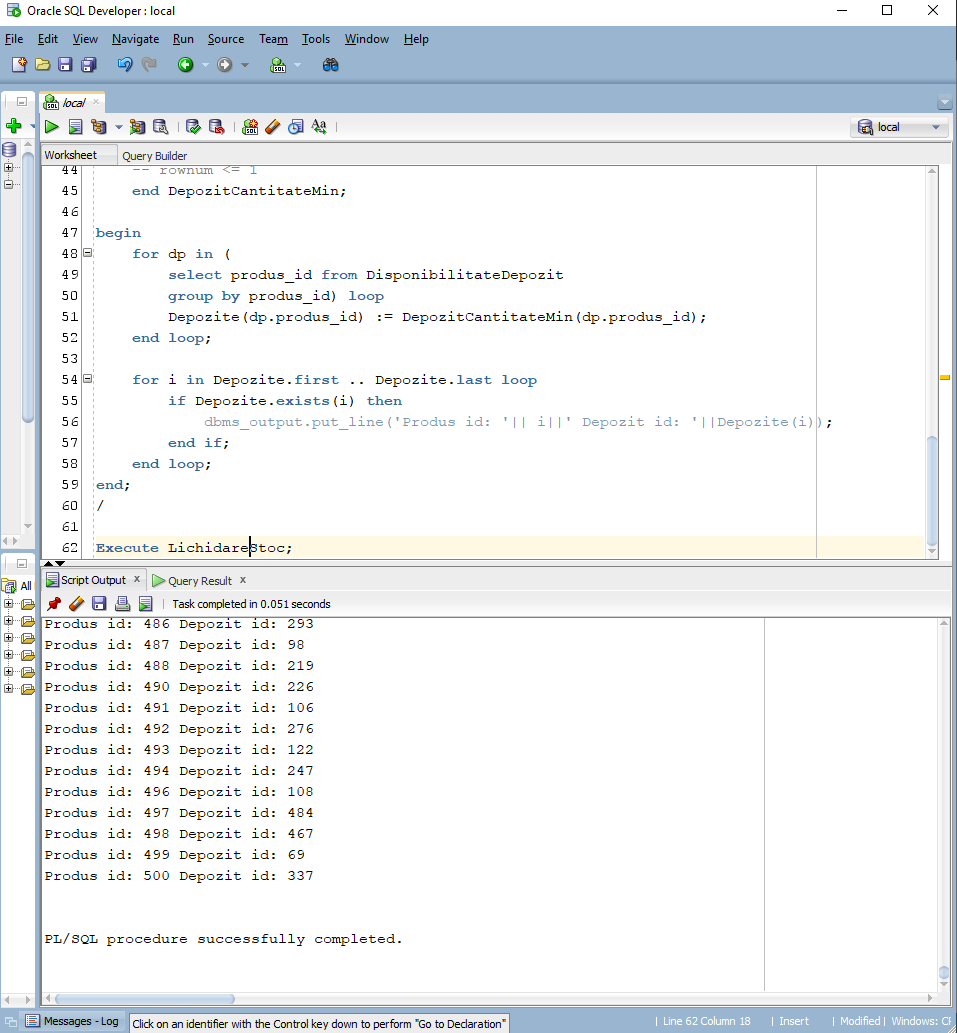
\includegraphics[width=1\linewidth]{Cerinta7.png}
\caption{Execuția cerinței 7}
\end{figure}

\begin{figure}[htp]
\centering
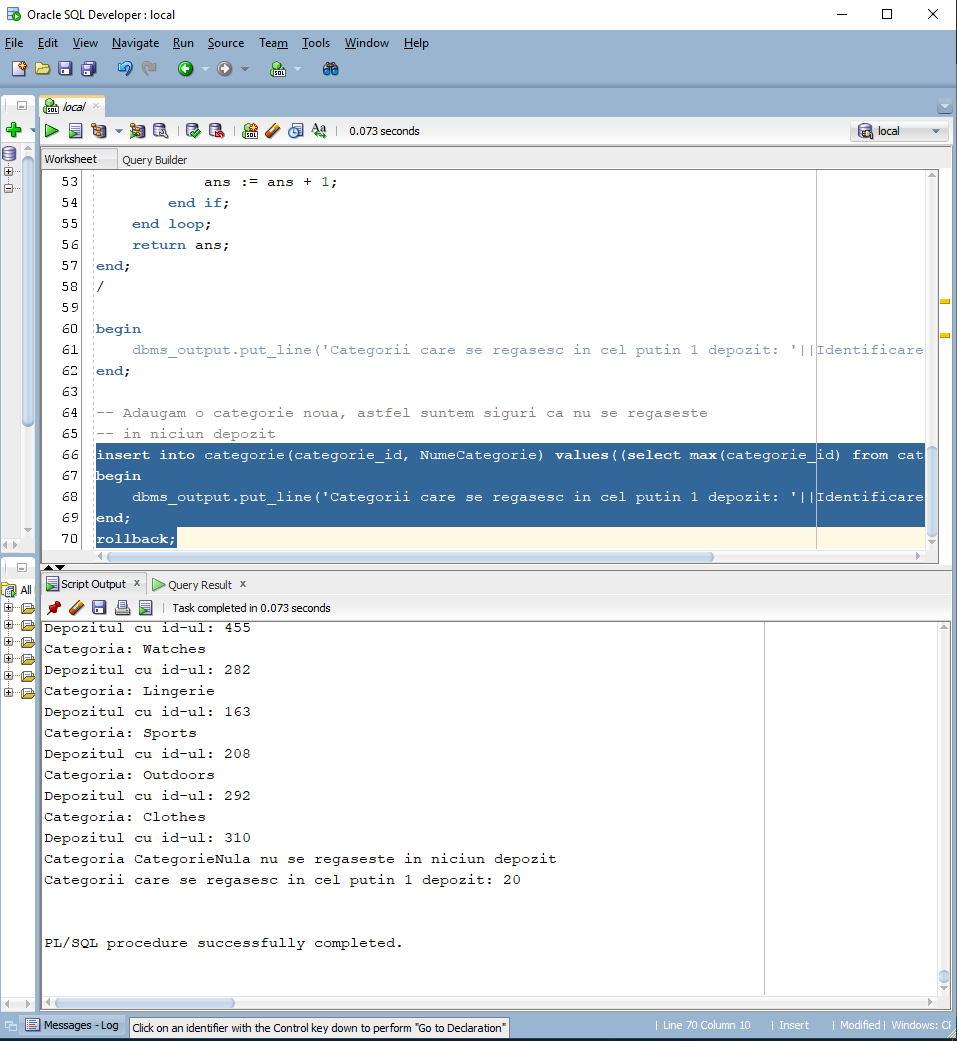
\includegraphics[width=1\linewidth]{Cerinta8.png}
\caption{Execuția cerinței 8}
\end{figure}

\begin{figure}[htp]
\centering
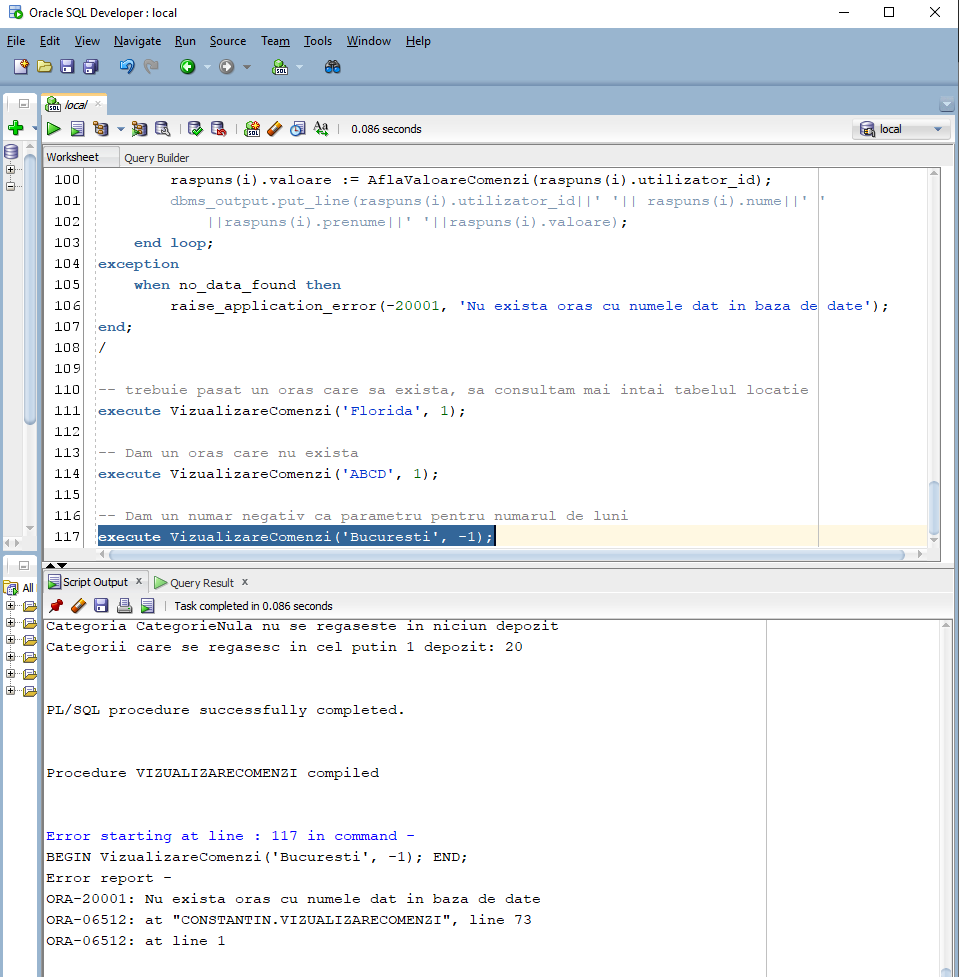
\includegraphics[width=1\linewidth]{Cerinta9.png}
\caption{Execuția cerinței 9}
\end{figure}

\begin{figure}[htp]
\centering
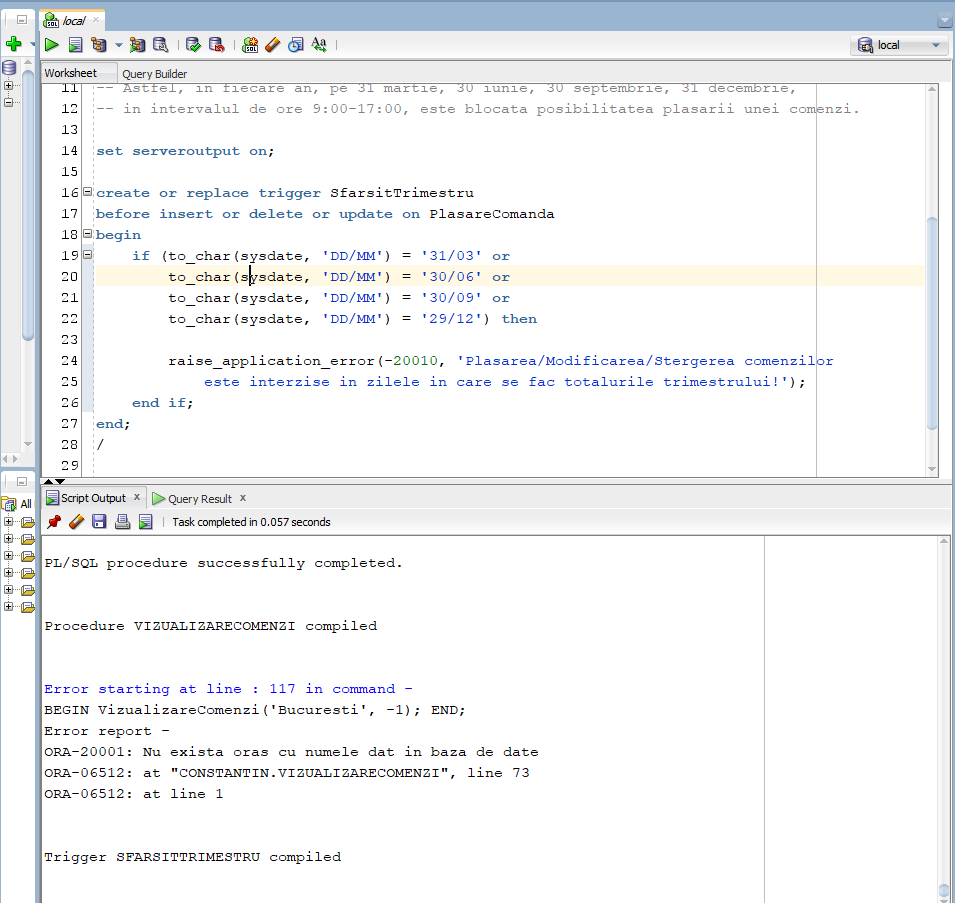
\includegraphics[width=1\linewidth]{Cerinta10.png}
\caption{Execuția cerinței 10}
\end{figure}

\begin{figure}[htp]
\centering
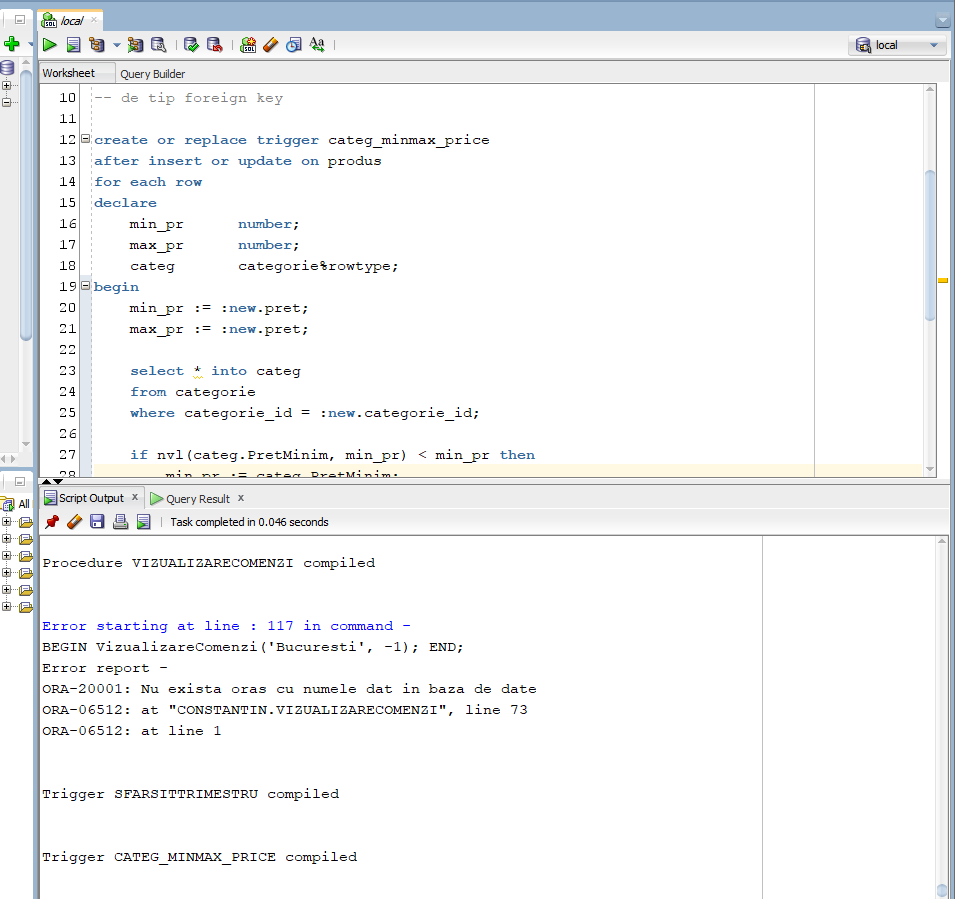
\includegraphics[width=1\linewidth]{Cerinta11.png}
\caption{Execuția cerinței 11}
\end{figure}

\begin{figure}[htp]
\centering
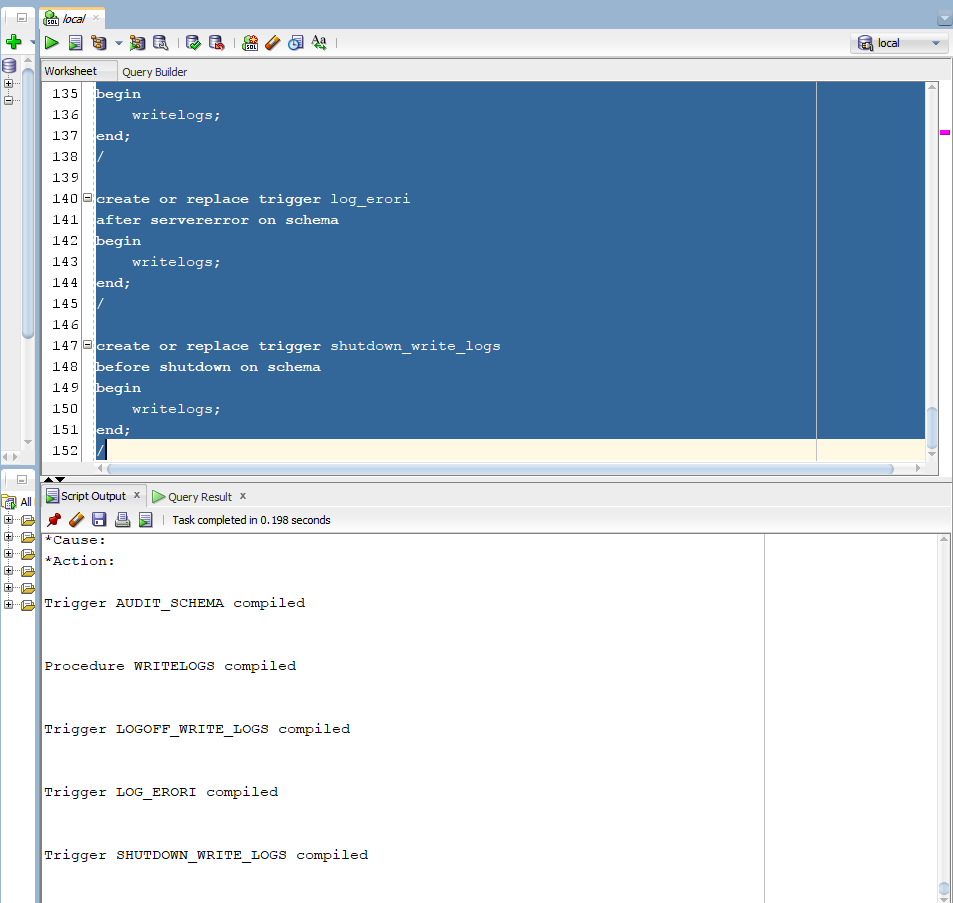
\includegraphics[width=1\linewidth]{Cerinta12.png}
\caption{Execuția cerinței 12}
\end{figure}

\begin{figure}[htp]
\centering
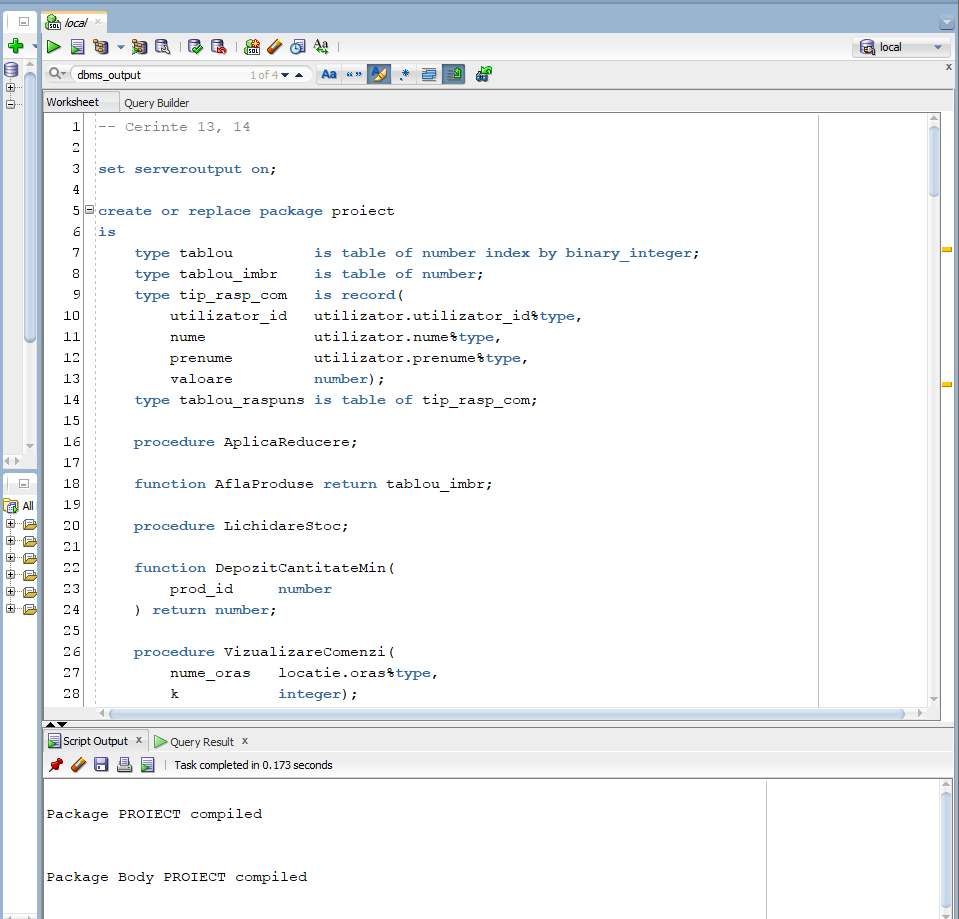
\includegraphics[width=1\linewidth]{Cerinta13.png}
\caption{Execuția cerinței 13}
\end{figure}

\begin{figure}[htp]
\centering
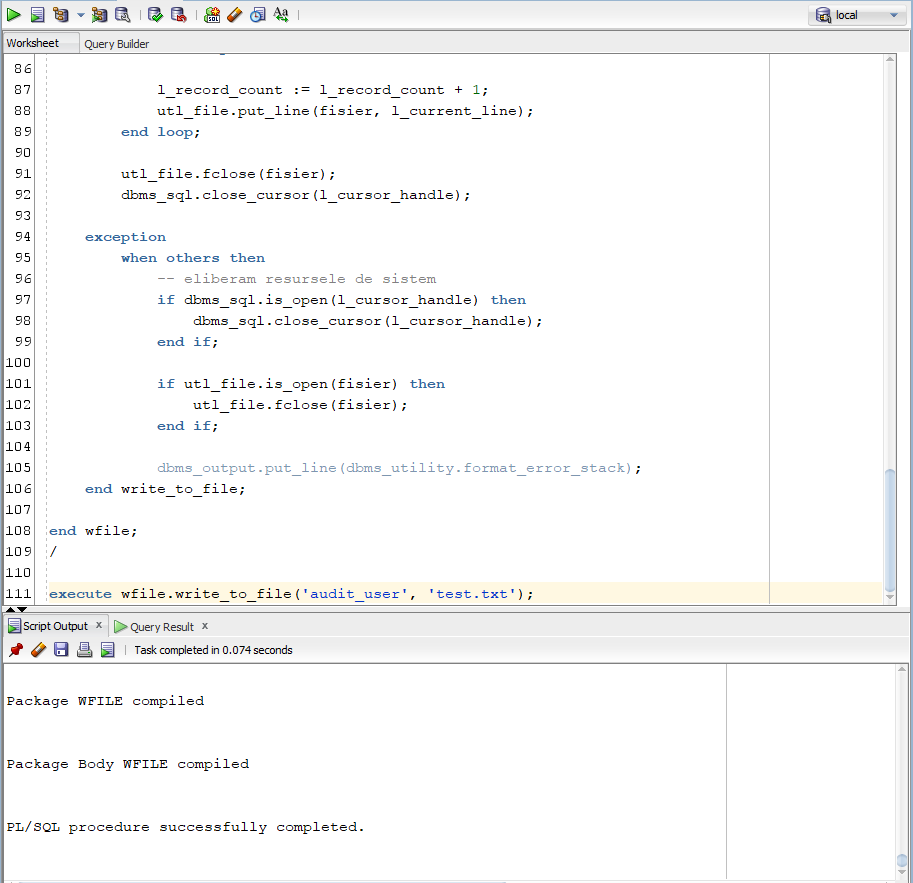
\includegraphics[width=1\linewidth]{Cerinta14.png}
\caption{Execuția cerinței 14}
\end{figure}

\bibliographystyle{abbrv}
\bibliography{main}

\end{document}